\documentclass[12pt]{article}

\usepackage{iftex}
\ifPDFTeX
    % Ћирилица: кодирање фонта и језик (српски, ћирилица)
    \usepackage[T2A]{fontenc}
    \usepackage[utf8]{inputenc}
    \usepackage[serbianc]{babel}
\else
    \usepackage{fontspec}
    \usepackage[serbian, english, bidi=basic, provide=*]{babel}
    \babelprovide[import, onchar=ids fonts]{serbian}
    \babelprovide[import, onchar=ids fonts]{english}
    \babelfont{rm}{Noto Sans}
\fi

% Величина стране и маргине
\usepackage[a4paper,top=2cm,bottom=2cm,left=2.5cm,right=2.5cm]{geometry}

% Корисни пакети
\usepackage{amsmath}
\usepackage{enumitem}
\usepackage{float}
\usepackage{booktabs}
\usepackage{tcolorbox}
\tcbuselibrary{breakable}
\usepackage[colorlinks=true, allcolors=blue]{hyperref}

% Цртање електричних кола (европски симболи)
\usepackage[european]{circuitikz}
\usetikzlibrary{babel}

% Оквир за решене примере
\newtcolorbox[auto counter]{primer}{breakable,
    colback=white, colframe=black!55, colbacktitle=black!55, coltitle=white,
    fonttitle=\bfseries\small, title={Пример~\thetcbcounter},
    boxrule=0.5pt, arc=1.5pt, left=6pt, right=6pt, top=3pt, bottom=3pt,
    before skip=8pt, after skip=10pt}

% Оквир за кључне делове и формуле
\newtcolorbox{kljucno}{breakable,
    colback=blue!4, colframe=blue!45!black,
    boxrule=0.5pt, arc=1.5pt, left=8pt, right=8pt, top=4pt, bottom=4pt}

\title{Bosch M-Motronic систем убризгавања и паљења - пропитивање}
\author{Аутоелектронски системи 2}
\date{}

\begin{document}
\maketitle

%##################################################################
\section{Bosch M-Motronic}
%##################################################################

За разлику од старијих Jetronic система (KE-Jetronic, L-Jetronic и
Mono-Jetronic), који су управљали искључиво убризгавањем горива, док је
систем паљења био потпуно одвојен, \textbf{M-Motronic} обједињује
\textbf{електронско убризгавање у више тачака (MPI)} и \textbf{електронску
контролу паљења} у једној заједничкој електронској управљачкој јединици
(ЕУЈ / CPU).

Потребне информације о раду мотора прикупљају се помоћу сензора и даље се
обрађују у заједничком микропроцесору. На основу свих информација и усклађених
тродимензионалних мапа за гориво и паљење, управљачка јединица истовремено
израђује управљачке сигнале за \textbf{електромагнетне бризгаљке, индукционе
калемове (бобине), регулатор празног хода, електрични (EVAP) вентил
регенератора, пумпу и вентил секундарног ваздуха, као и вентил за повраћај
издувних гасова (EGR)}.

Сваки цилиндар има сопствену електромагнетну бризгаљку смештену испред
усисног вентила (MPI). Бризгаљка је електромагнетни вентил, а количину
убризганог горива одређује управљачка јединица дужином импулса, тј. временом
за које држи бризгаљку отвореном. Истовремено, рачунар за сваки радни такт
израчунава оптималан угао претпаљења и време пуњења бобине, чиме се угао
паљења и дозирање горива усклађују у сваком режиму рада мотора.

\begin{kljucno}
\begin{enumerate}[noitemsep]
    \item[1.] Регенератор са активним угљем
    \item[2.] Вентил за ваздух
    \item[3.] Електрични (EVAP) вентил регенератора
    \item[4.] Регулатор притиска за гориво
    \item[5.] Бризгаљка
    \item[6.] Регулатор притиска у усисној цеви
    \item[7.] Индукциони калем -- бобина
    \item[8.] Сензор фазе
    \item[9.] Пумпа за секундарни ваздух
    \item[10.] Вентил секундарног ваздуха
    \item[11.] Мерач протока ваздуха -- протокомер
    \item[12.] Електронска или централна управљачка јединица (CPU)
    \item[13.] Давач положаја пригушног лептира
    \item[14.] Регулатор празног хода
    \item[15.] Сензор температуре ваздуха
    \item[16.] Вентил за повраћај (рециркулацију) издувних гасова
    \item[17.] Филтер за гориво
    \item[18.] Сензор кликтања
    \item[19.] Сензор броја обртаја мотора
    \item[20.] Сензор температуре мотора
    \item[21.] ЛАМБДА сонда
    \item[22.] Прикључак за дијагностику
    \item[23.] Сигнална лампица прикључка
    \item[24.] Сензор разлике притиска
    \item[25.] Резервоар за гориво са уграђеном електричном пумпом
\end{enumerate}
\end{kljucno}

\begin{figure}[H]
    \centering
    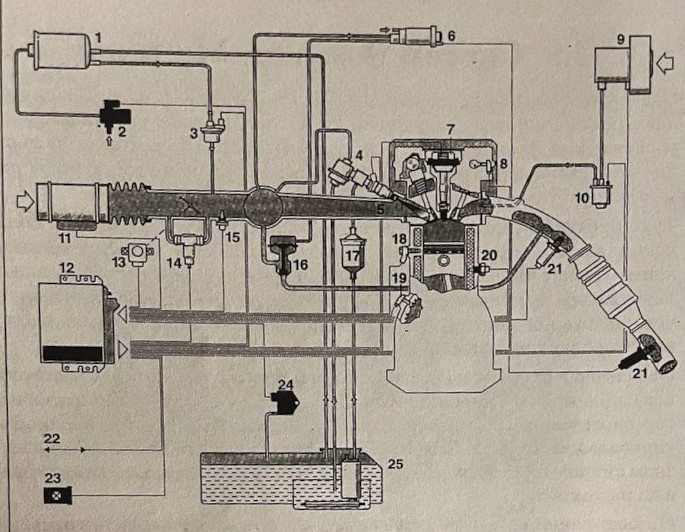
\includegraphics[width=0.7\textwidth]{slike/1.jpg}
    \caption{Опис слике који се приказује испод}
    \label{fig:naziv-slike}
\end{figure}

%##################################################################
\section{Шта решава и по коју цену}
%##################################################################

Код старијих система у којима су убризгавање и паљење били раздвојени, није
постојала непосредна размена података између та два система. Механички
разводник паљења са центрифугалним теговима и вакуумским коректором није могао
довољно прецизно да прати нагле промене оптерећења и квалитет горива, што је
ограничавало степен компресије, економичност и ефикасност трокомпонентног
катализатора.

M-Motronic решава ове недостатке обједињавањем свих функција под контролом
једног рачунара:

\begin{itemize}[noitemsep]
    \item \textbf{јединствено управљање убризгавањем и паљењем}: оба система
          користе исте сензоре и заједничке мапе, па се количина горива и угао
          претпаљења усклађују у сваком радном такту,
    \item \textbf{прецизно убризгавање у више тачака (MPI)}: сваки цилиндар
          добија одмерену количину горива непосредно испред усисног вентила,
          без таложења горивног филма на зидовима усисног колектора,
    \item \textbf{активна регулација кликтања}: захваљујући сензору кликтања,
          угао претпаљења се одржава на самој граници детонације ради веће
          ефикасности, а при појави кликтања тренутно се смањује за
          појединачни цилиндар,
    \item \textbf{строга контрола емисије издувних гасова}: поред прецизне
          ЛАМБДА регулације ($\lambda = 1$), систем управља и удувавањем
          секундарног ваздуха (брзо загревање катализатора) и рециркулацијом
          издувних гасова (смањење $\text{NO}_x$).
\end{itemize}

\textbf{Цена} овако високе прецизности и еколошке чистоће је већа сложеност
и виша цена самог система:

\begin{itemize}[noitemsep]
    \item већи број сензора и извршних органа (протокомер, сензор радилице,
          сензор фазе, сензор кликтања, појединачне бризгаљке, систем
          секундарног ваздуха, EGR вентил),
    \item сложенија електрична инсталација и вишеполни конектор управљачке
          јединице са великим бројем извода,
    \item захтевнија дијагностика и одржавање у случају квара неког од
          елемената, због чега је уграђена самодијагностика са меморијом
          грешака и прикључком за дијагностику.
\end{itemize}

\subsection{Мерење броја обртаја и угаоног положаја радилице}

На коленастом вратилу (радилици) или замајцу налази се импулсни венац са
\textbf{60 минус 2 зуба}. Пошто пун круг износи $360^\circ$, један корак
(зуб и удубљење) заузима $6^\circ$, односно по $3^\circ$ за узлазну и силазну
ивицу сигнала. Софтверском временском интерполацијом управљачка јединица
дели интервал од $3^\circ$ на 4 једнака дела, чиме постиже угаону резолуцију
од $0,75^\circ$.

Два недостајућа зуба служе као референтна тачка на основу које рачунар
препознаје тачан положај клипова у односу на горњу мртву тачку (ГМТ). Време
између два узастопна паљења назива се \textbf{временски сегмент} и одговара
углу $720^\circ / z$, где је $z$ број цилиндара (за четвороцилиндрични мотор
то је $180^\circ$, односно 30 зуба; за шестоцилиндрични $120^\circ$, а за
осмоцилиндрични $90^\circ$). У комбинацији са \textbf{сензором фазе} на
брегастом вратилу, рачунар разликује такт сабијања од такта издувавања, што
омогућава секвенцијално убризгавање и директно паљење без класичног
разводника.

\subsection{Регенерација бензинских пара, секундарни ваздух и EGR}

Прописи о заштити животне средине захтевају строго ограничење емисије
штетних гасова у свим режимима рада мотора. Поред одржавања идеалне смеше
($\lambda = 1$) за рад трокомпонентног катализатора, M-Motronic управља са
три додатна еколошка подсистема:

\begin{itemize}[noitemsep]
    \item \textbf{Регенерација и утрошак бензинских пара (EVAP):} Регенератор
          са активним угљем упија бензинске паре из резервоара. Када
          електрични EVAP вентил отвори пролаз по команди рачунара,
          потпритисак у усисној цеви повлачи свеж ваздух кроз канистер у
          супротном смеру и одводи упијено гориво у цилиндре на сагоревање.
    \item \textbf{Удувавање секундарног ваздуха (SAI):} При хладном старту
          мотора, када је смеша обогаћена а катализатор још хладан, електрична
          пумпа преко вентила секундарног ваздуха убацује свеж кисеоник
          директно у издувну грану. Тиме се изазива накнадно сагоревање
          несагорелих угљоводоника ($\text{HC}$) и угљен-моноксида
          ($\text{CO}$), а ослобођена топлота убрзава загревање катализатора на
          радну температуру ($300\text{--}400\,^\circ\text{C}$).
    \item \textbf{Повраћај дела издувних гасова (EGR):} При делимичном
          оптерећењу мотора, EGR вентил враћа део већ сагорелих издувних гасова
          из издувне у усисну грану. Инертни гасови разблажују свежу смешу и
          снижавају максималну температуру сагоревања у цилиндру, чиме се
          значајно смањује стварање азотних оксида ($\text{NO}_x$). На празном
          ходу, код хладног мотора и при пуном оптерећењу вентил је затворен.
\end{itemize}

\subsection{Регулација кликтања и прекопчавање усисног вода}

\begin{itemize}[noitemsep]
    \item \textbf{Сензор кликтања} је пиезоелектрични давач причвршћен на блок
          мотора који детектује високофреквентне вибрације услед детонантног
          сагоревања. Када региструје кликтање у поједином цилиндру, рачунар
          тренутно смањује угао претпаљења за тај цилиндар, а након престанка
          детонација постепено га враћа ка оптималној вредности.
    \item \textbf{Прекопчавање усисног вода} (усисна грана променљиве дужине)
          помоћу заклопки којима управља рачунар мења путању ваздуха до
          цилиндара: на ниским обртајима ваздух струји дужим каналом ради
          коришћења таласа притиска (резонантно пуњење и већи обртни момент),
          док се на високим обртајима отвара краћи пут за максималну снагу.
\end{itemize}

\subsection{Симултано и секвенцијално убризгавање}

Код система са убризгавањем у више тачака (MPI) разликују се два основна
начина активирања бризгаљки. Код \textbf{симултаног убризгавања} (карактеристичног
за старији L-Jetronic), све бризгаљке се отварају истовремено -- једном или двапут
током радног циклуса, независно од тога који се цилиндар тренутно налази у такту
усисавања. Овакав приступ поједностављује управљачку електронику и не захтева
сензор фазе, али се гориво код појединих цилиндара задржава испред затвореног
усисног вентила. Насупрот томе, \textbf{секвенцијално убризгавање} (примењено код
M-Motronic система) подразумева да рачунар управља сваком бризгаљком посебно и
убризгава гориво редом, према редоследу паљења, непосредно пре отварања усисног
вентила одговарајућег цилиндра. За овакав рад неопходан је \textbf{сензор фазе}
на брегастом вратилу, а предности су уједначенији састав смеше у свим
цилиндрима, бржи одзив на педалу гаса, као и мања потрошња горива и емисија
штетних гасова.

\begin{figure}[H]
    \centering
    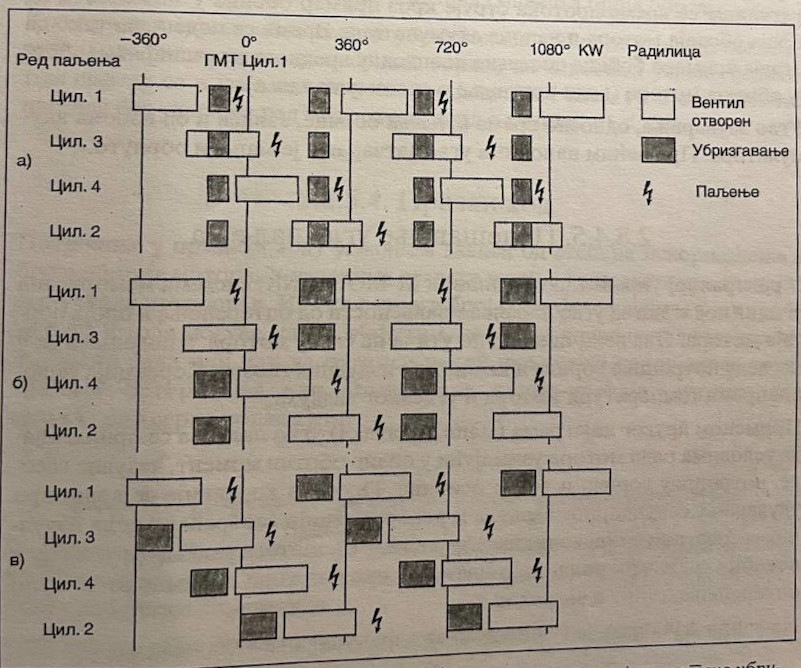
\includegraphics[width=0.7\textwidth]{slike/11.jpg}
    \caption{Опис слике који се приказује испод}
    \label{fig:naziv-slike}
\end{figure}

\section{Поређење M-Motronic система са L-Jetronic и Mono-Jetronic системима}

Развојно гледано, \textbf{M-Motronic} представља обједињавање и надоградњу
претходних Bosch система: од \textbf{L-Jetronic} система преузима принцип
убризгавања у више тачака (MPI) и директно мерење количине усисаног ваздуха,
док од дигиталних система попут \textbf{Mono-Jetronic-а} преузима микропроцесорску
обраду података са тродимензионалним мапама и адаптивном ЛАМБДА регулацијом,
спајајући притом \textbf{убризгавање горива и паљење у једну управљачку јединицу}.

\subsection{Шта је заједничко, а шта ново у односу на L-Jetronic}

\textbf{L-Jetronic} и \textbf{M-Motronic} деле исту основну хидрауличну
концепцију припреме смеше: оба система имају по једну електромагнетну бризгаљку
испред усисног вентила сваког цилиндра (MPI), раде под сличним притиском горива
(око $2{,}5\text{--}3{,}5\text{ bar}$) који се одржава помоћу вакуумског регулатора
притиска, и директно мере количину ваздуха који улази у мотор.

Међутим, M-Motronic доноси кључна унапређења у односу на L-Jetronic:

\begin{itemize}[noitemsep]
    \item \textbf{Интеграција паљења:} L-Jetronic управља искључиво убризгавањем
          горива, док је паљење потпуно одвојено (разводник са центрифугалним
          теговима и вакуумским коректором). M-Motronic управља и убризгавањем
          и углом претпаљења из истог микропроцесора.
    \item \textbf{Дигитална електроника уместо аналогне:} L-Jetronic користи
          претежно аналогна електронска кола, док M-Motronic користи дигитални
          микропроцесор са меморијама (EPROM/Flash и RAM), прецизним мапама и
          самодијагностиком.
    \item \textbf{Регулација кликтања:} L-Jetronic нема заштиту од детонација,
          док M-Motronic помоћу сензора кликтања може појединачно по цилиндру
          да враћа угао претпаљења при појави детонација.
    \item \textbf{Мерење ваздуха и обртаја:} Уместо механичке мерне заклопке
          (потенциометра протокомера) код L-Jetronic-а, M-Motronic користи
          савременији мерач масе ваздуха (са ужареном жицом или филмом), а
          уместо импулса са бобине/разводника користи импулсни венац на
          радилици ($60-2$ зуба) и сензор фазе.
    \item \textbf{Поједностављен хладан старт и празан ход:} M-Motronic избацује
          посебну бризгаљку за хладан старт и термовременски прекидач (обогаћење
          врши продужењем импулса главних бризгаљки), а биметални вентил за
          додатни ваздух замењује електронским регулатором празног хода.
\end{itemize}

\subsection{Шта је промењено у односу на Mono-Jetronic}

Док је \textbf{Mono-Jetronic} пројектован као јефтина замена за карбуратор са
једном централном бризгаљком (SPI) и посредним рачунањем ваздуха из угла лептира
($\alpha$) и броја обртаја ($n$), M-Motronic прелази на знатно прецизније и
сложеније решење:

\begin{itemize}[noitemsep]
    \item уводи се по једна бризгаљка за сваки цилиндар (MPI) и већи притисак
          горива, чиме се избегава таложење филма горива у усисној грани,
    \item уводи се директно мерење протока ваздуха (протокомер),
    \item укида се класичан разводник паљења и уводи електронска контрола
          угла претпаљења са сензором радилице ($60-2$) и сензором кликтања,
    \item поред EVAP вентила, додају се системи за удувавање секундарног
          ваздуха и рециркулацију издувних гасова (EGR).
\end{itemize}

\begin{table}[H]
    \centering
    \footnotesize
    \renewcommand{\arraystretch}{1.3}
    \begin{tabular}{p{2.7cm} p{3.3cm} p{3.3cm} p{3.7cm}}
        \toprule
        \textbf{Карактеристика} & \textbf{L-Jetronic} & \textbf{Mono-Jetronic} & \textbf{M-Motronic} \\
        \midrule
        Тип убризгавања & више тачака (MPI) & једна тачка -- централно (SPI) & више тачака (MPI), секвенцијално \\
        \midrule
        Управљање паљењем & одвојено (разводник са теговима/вакуумом) & одвојено (разводник са теговима/вакуумом) & интегрисано у исти рачунар (CPU) \\
        \midrule
        Електроника ЕУЈ & претежно аналогна & дигитална (само за гориво) & дигитална (гориво + паљење + екологија) \\
        \midrule
        Мерење ваздуха & директно (мерна заклопка) & посредно (угао лептира $\alpha$ и обртаји $n$) & директно (протокомер -- жица / филм) \\
        \midrule
        Притисак горива & око $2{,}5\text{--}3{,}5\text{ bar}$ & око $1\text{ bar}$ & око $2{,}5\text{--}4\text{ bar}$ \\
        \midrule
        Давач обртаја и положаја & импулси са система паљења / разводника & Холов давач у разводнику паљења & сензор радилице ($60-2$) + сензор фазе \\
        \midrule
        Хладан старт & посебна бризгаљка + термовременски прекидач & продужење импулса главне бризгаљке & продужење импулса главних бризгаљки \\
        \midrule
        Празан ход & биметални вентил додатног ваздуха & корачни мотор помера сам лептир & електромагнетни регулатор празног хода \\
        \midrule
        Заштита од детонација & нема & нема & сензор кликтања (по цилиндру) \\
        \midrule
        Еколошки подсистеми & нема (или основна $\lambda$-регулација) & ЛАМБДА сонда + EVAP вентил & ЛАМБДА + EVAP + секундарни ваздух + EGR \\
        \bottomrule
    \end{tabular}
    \caption{Упоредни преглед система L-Jetronic, Mono-Jetronic и M-Motronic}
\end{table}

%##################################################################
\section{Електронска управљачка јединица}
%##################################################################
\begin{kljucno}
\begin{itemize}
    \item Маса управљачке јединице изведена је преко одвојених извода.
          Електронски део за пријем осетљивих сигнала (NTC сензори температуре,
          ЛАМБДА сонда, потенциометар лептира, сензор кликтања) има посебну
          сензорску масу, док посебна енергетска маса служи за извршне органе
          кроз које теку веће струје.
    \item Везе са ЛАМБДА сондом, сензором броја обртаја и сензором кликтања
          изведене су оклопљеним (ширмованим) кабловима, да би се спречиле
          индуктивне сметње од система паљења и других струјних кола.
    \item Пумпа за гориво напаја се преко посебног релеја којим управља
          јединица. По укључењу контакт-кључа пумпа ради неколико секунди да
          подигне притисак у систему. Ако мотор престане да ради (изостану
          импулси са сензора броја обртаја, нпр. после незгоде), релеј
          аутоматски прекида напајање пумпе.
\end{itemize}
\end{kljucno}

\begin{figure}[H]
    \centering
    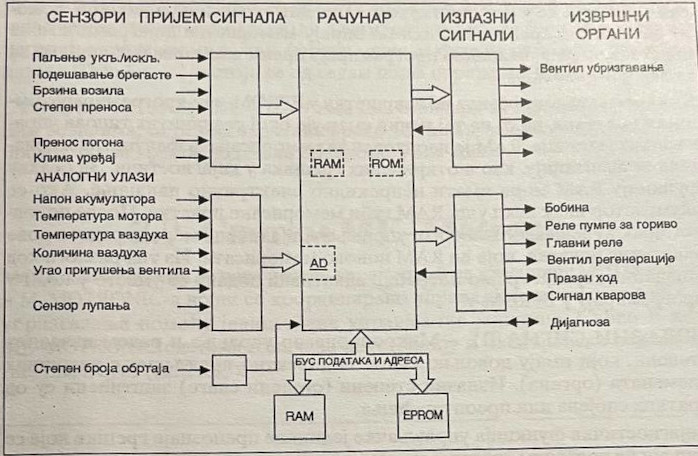
\includegraphics[width=0.7\textwidth]{slike/16.jpg}
    \caption{Опис слике који се приказује испод}
    \label{fig:naziv-slike}
\end{figure}

%##################################################################
\section{Обрада података}
%##################################################################

\begin{kljucno}
Прикупљени подаци са сензора доводе се до управљачке јединице, која их
прилагођава и обрађује. Према уграђеном програму јединица израђује
управљачке сигнале за бризгаљке, индукционе калемове (бобине), регулатор
празног хода, EVAP вентил, EGR вентил и пумпу секундарног ваздуха.
\end{kljucno}

\begin{kljucno}
\begin{itemize}
    \item \textbf{Аналогно-дигитални претварач.} Аналогни сигнали (протокомер,
          напон ЛАМБДА сонде, отпор потенциометра лептира, напон давача
          температуре, напон акумулатора) претварају се у дигиталне вредности
          које микропроцесор може да обради. Импулсни сигнали са сензора
          радилице и сензора фазе обликују се посебним улазним колом.
    \item \textbf{Микропроцесор} прима податке од сензора преко интерфејса и
          А/Д претварача и, према програму, израчунава време отварања
          бризгаљки и угао претпаљења. Повезан је са меморијом
          \textbf{EPROM / Flash}, у којој су програм и тродимензионалне мапе,
          и са меморијом \textbf{RAM}, у коју се уписују адаптивне корекције
          смеше и кодови грешака за дијагностику. Да се подаци не би изгубили
          после гашења мотора, RAM је стално повезан са акумулатором.
    \item \textbf{Излазни степени} су појачавачи са транзисторима снаге, преко
          којих микропроцесор управља бризгаљкама, примарним колима бобина,
          регулатором празног хода, EVAP и EGR вентилом, релејима пумпи и
          сигналном лампицом дијагностике.
\end{itemize}
\end{kljucno}

%##################################################################
\section{Прилагођавање раду мотора}
%##################################################################

Управљачка јединица прилагођава убризгавање горива и угао паљења следећим
режимима и условима рада:
\begin{itemize}[noitemsep]
    \item хладан старт,
    \item загревање мотора (обогаћење смеше и удувавање секундарног ваздуха),
    \item температура усисаног ваздуха,
    \item празан ход,
    \item делимично оптерећење (активирање EGR система),
    \item пуно оптерећење,
    \item регулација кликтања по појединачном цилиндру,
    \item ограничење броја обртаја,
    \item кочење мотором (прекид довода горива),
    \item принудна вожња у случају квара (Limp-Home режим),
    \item компензација у прелазним режимима,
    \item ЛАМБДА регулација ($\lambda = 1$),
    \item адаптација радне смеше,
    \item компензација пада напона акумулатора.
\end{itemize}

\end{document}